\newpage
\visHeader

\begin{itemize}
\FloatBarrier
\item[$\blacktriangleright$] Did you notice the new Demo.eap file in your project explorer? This is the EA file you'll be testing and modelling your program with. Don't worry about the other folder and the exclamation mark it carries. In the next step, you'll resolve that error.

In the meantime, Please do not rename, move, or delete anything.

% THIS NEEDS AN IMAGE
\item[$\blacktriangleright$] Press the small arrow in the package explorer, and choose working sets as your top level element (Fig.~\ref{fig_eclipseWorkingsets}). We work a lot with working sets, and use them to structure the workspace in Eclipse.

\item[$\blacktriangleright$] Double click ``Demo.eap'' to start EA, and choose ``Ultimate" when starting EA for the first time.

\item[$\blacktriangleright$] In EA, choose ``Extensions/MOFLON::Ecore Addin/Export\- all\- to\- Workspace'' (Fig.~\ref{fig_ea}).
You can of course browse the project structure, but please do not rename, move, or delete anything yet.

\begin{figure}[htbp]
	\centering
  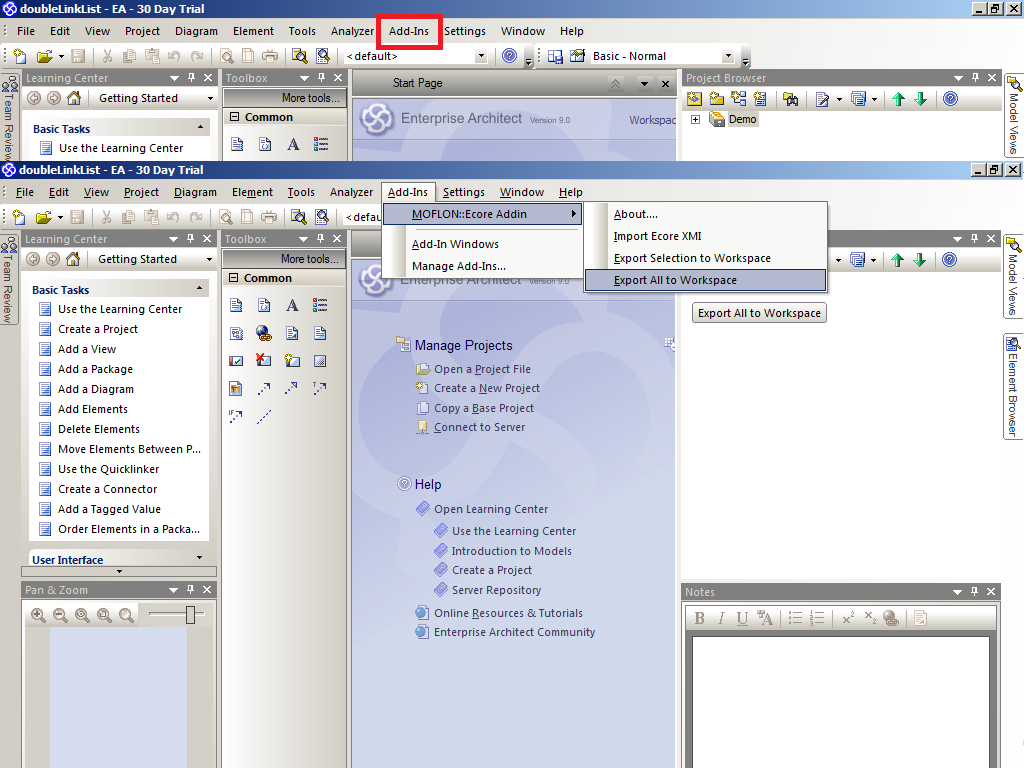
\includegraphics[width=0.9\textwidth]{ea_firststart}
	\caption{Export from EA using our extension} 
	\label{fig_ea} 
\end{figure}
  
\item[$\blacktriangleright$] Switch back to Eclipse, choose your Metamodel project, and press F5 to refresh.
The export from EA places all required files in a hidden folder in the project, and refreshing triggers a build process that invokes our code generators automatically.
You should be able to monitor the progress in the lower right corner (Fig.~\ref{fig_eclipsebuilding}).  
Pressing the symbol opens a monitor view that gives more details of the build process. 
You don't need to worry about any of these details, just remember to refresh your Eclipse workspace after an export.
\end{itemize}